\documentclass{article}
\usepackage[utf8]{inputenc}
% Se importa el paquete.
\usepackage{listings}
\usepackage{color}
\usepackage{fullpage}
\usepackage[english]{babel}
\usepackage[utf8]{inputenc}
\usepackage{amsmath,amsthm,amssymb,amsfonts,mathrsfs,latexsym,stmaryrd}
\usepackage{color} 
\usepackage{graphicx}
\usepackage{textpos}

% Definición lenguaje.
\newcommand{\CommentColor}{\color{green!60!black}}
\newcommand{\StringColor}{\color{red!70!black}}
\newcommand{\UserKeywordsColor}{\color{cyan!50!black}}
\newcommand{\KeywordsColor}{\color{blue}}

\lstdefinelanguage{Assemblyx86}
{
  basicstyle=\small\ttfamily,
  keywordstyle=\KeywordsColor\textbf,
  keywordstyle=[2]\StringColor,
  keywordstyle=[3]\UserKeywordsColor,
  tabsize=4,
  morekeywords={MOV, PUSH, POP, ADD, SUB, MUL, POPA, PUSHA, IRET, 
    DIV, INC, DEC, CMP, NOT, AND, OR, XOR, INT,
    LEA, CALL, RET, JMP, JE, JNE, JG, JGE, JL, JLE, IN, OUT, SHR, SHL, JEQ, MULPS, ADDPS},
  morekeywords=[2]{A,B,AX,AH,AL,BX,BH,BL,CX,CH,CL,DX,DH,DL,SI,DI,SP,BP},
  morekeywords=[3]{db,dw}, 
  commentstyle=\CommentColor,
  stringstyle=\StringColor,
  sensitive=true,
  morecomment=[l]{;},
  morecomment=[s]{/*}{*/},
  morestring=[b]",
  showstringspaces=false,
  aboveskip=0pt, 
  belowskip=0pt,
  mathescape=true
}

% Comienzo documento.
\begin{document}

% Se setea el lenguaje.
\lstset{language=Assemblyx86}

% Se crea un listing (fragmento de código). Con frame = single se crea un borde que rodea al código.

            TAREA 7


Vicente VIAL 

14621045


A)




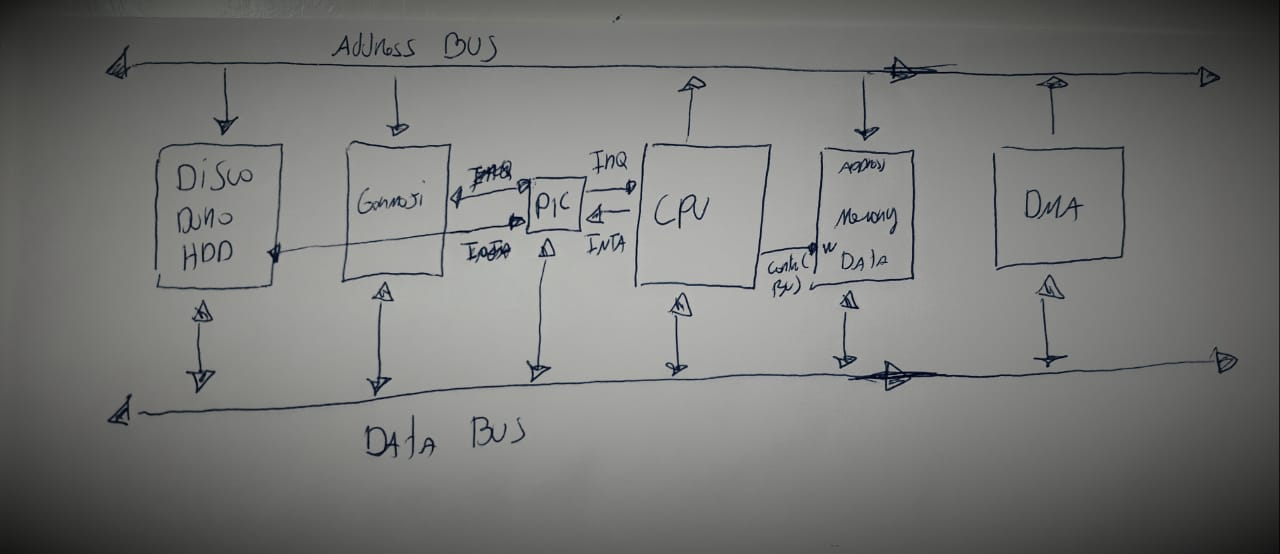
\includegraphics[width=20cm]{foto.jpeg}
 



B)

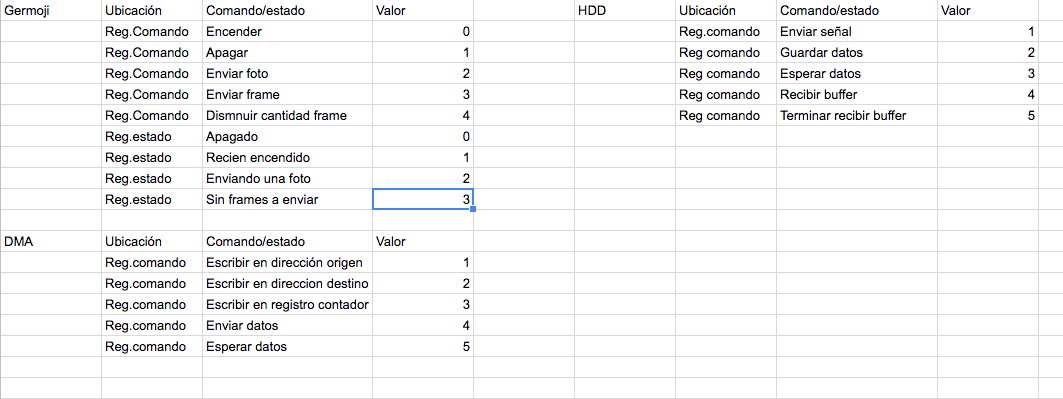
\includegraphics[width=18cm]{foto1.png}



    \begin{lstlisting} 
    
C)



PRIMERA OPCION:

   ISR9:
       IN BX, 0x06 ; se ve estado de dispositivo
       CMP BX,0x00 ; se revisa si estado es apagado o prendido
       JNE empeza ; Si esta apagado prender
       OUT (0X06) , 1 ; cambio a encendido
       empezar:
       MOV DX, [0XCC26]  ; almacena datos de cantidad de frames a enviar
       CMP DX, Ox00 ; reviso si quedan frames a enviar
       JE retorna ; si no quedan frames a enviar retorno
       OUT (0X06) , 2; cambio a enviando foto
       MOV BX, 38 ; registro en  BX la primera posicion del  Buffer rojo
       enviar_frames:
        MOV Dx, [0xCC26] ; usare Dx como contador
        IN Cx, 0x0007 ; reviso comando DMA
        CMP Cx, 5 ; 
        JNE,  enviar_frames ; si su comando no es esperar datos, entonces se espera a que se cambie
        MOV AX, 0x0926 ; registro en AX inicio de buffer de disco duro
        enviar_pixeles: ; se envian pixeles
        MOV CX, [BX] ; guardo en CX, valor de comienzo de BX
        MOV [AX], [BX] ; registro en buffer disco duro,  pixel de canal rojo
        ADD AX, 1
        ADD Bx, 768
        MOV [AX], [BX] ; registro en buffer de disco duro pixel de canal verde
        ADD AX, 1
        ADD Bx, 768
        MOV [AX], [BX] ; registro en buffer de disco duro pixel de canal azul
        ADD AX, 1
        MOV BX, CX
        ADD BX, 1
        CMP BX, 806   ; ¿se envio frame completo?
        JNE envio_completo_frame
        enviar_pixeles
        envio_completo_frame:
        CMP DX, 0X0000 ; compruebo si se han enviado todos los frames
        JE, empezar
        SUB DX, 0X0001
        OUT (0x0007), 4; actualizo comando DMA enviar 
        enviar_frames
        retornar:
        OUT (0X06) , 3
        IRET
    \end{lstlisting}
       
       
       
    \begin{lstlisting} 

SEGUNDA OPCION:

   ISR10:
       IN BX, 0x06 ; se ve estado de dispositivo
       CMP BX,0x00 ; se revisa si estado es apagado o prendido
       JNE empeza ; Si esta apagado prender
       OUT (0X06) , 1 ; cambio a encendido
       empezar:
       MOV DX, [0XCC26]  ; almacena datos de cantidad de frames a enviar
       CMP DX, Ox00 ; reviso si quedan frames a enviar
       JE retorna ; si no quedan frames a enviar retorno
       OUT (0X06) , 2; cambio a enviando foto
       MOV BX, 38 ; registro en  BX la primera posicion del  Buffer rojo
       enviar_frames:
        MOV Dx, [0xCC26] ; usare Dx como contador
        ; se elimia esta parte, primer cambio
        MOV AX, 3110 ; registro en AX inicio de memoria libre
        enviar_pixeles: ; se envian pixeles
        MOV CX, [BX] ; guardo en CX, valor de comienzo de BX
        MOV [AX], [BX] ; registro en buffer disco duro,  pixel de canal rojo
        ADD AX, 1
        ADD Bx, 768
        MOV [AX], [BX] ; registro en buffer de disco duro pixel de canal verde
        ADD AX, 1
        ADD Bx, 768
        MOV [AX], [BX] ; registro en buffer de disco duro pixel de canal azul
        ADD AX, 1
        MOV BX, CX
        ADD BX, 1
        CMP BX, 806   ; ¿se envio frame completo?
        JNE envio_completo_frame
        enviar_pixeles
        envio_completo_frame:
        CMP DX, 0X0000 ; compruebo si se han enviado todos los frames
        JE, retornar ; segundo cambio, se retorna despues de mandar todos los frames
        SUB DX, 0X0001
        OUT (0x0007), 4; actualizo comando DMA enviar 
        enviar_frames
        retornar:
        OUT (0X06) , 3
        IRET
    \end{lstlisting}
       
       
       
       
       
       
       
       
       

    
    
        ;d) Para este caso se usará la segunda opcion de Geremy, que retorna despues de enviar los 3 frames   
    
    \begin{lstlisting} 
    OUT (0X0007), 2
    OUT (0X0008), 5
    OUT (0X000C), 3 
    ;SETEO ESTADOS PRIMERO
    ;ASUMO QUE SE APRETO ENVIAR FOTO
    
    
    program:
      IN Ax, (0x0007) ; se revisa si comando es   enviar
      CMP Ax, 2; ¿enviar?
      JNE program
      OUT (0x0006), 2 ; se actualiza estado a enviar
      
       empezar:
       MOV DX, [0XCC26]  ; almacena datos de cantidad de frames a enviar
       CMP DX, Ox00 ; reviso si quedan frames a enviar:
       JE retorna ; si no quedan frames a enviar retorno
       INT10 ; se llama a geremy_2
       MOV BX, 3110 ; se usara despues
       traspaso_dma_a_HHD:
       IN AX, (0X000C)
       CMP AX,2 ; ¿guardar datos?
       JE guardar_datos_HHDD
       IN Ax, (0x0008) ; se revisa si comando es enviar
       CMP AX, 4 ; ¿enviar?
       JE, enviar_datos_HDD
       JMP traspaso_dma_a_HDD
       guardar_datos_HHDD:
       INT 8
       OUT (0X000C), 3 
       JMP traspaso_dma_a_HDD
       enviar_datos_HDD:
       MOV AX, 2342
       traspaso_a_buffer:
       MOV [AX], [BX]  ; guardo en AX, imagen guardada en memoria
       ADD AX, 1
       ADD BX, 1
       CMP BX, 3877
       JE termino_frame
       CMP BX, 4644
       JE termino_frame
       CMP BX, 5411
       JE termino_frame_final
       JMP traspaso_a_buffer
       
       termino_frame:
       IN (0X000C), 2 ; cambio a guardar datos
       OUT (0X0009), 2342
       OUT (0X000B), 767
       INT 7
       JMP traspaso_dma_a_HHDD
       
       
       termino_frame_final:
       OUT (0X0009), 2342
       OUT (0X000B), 767
       INT 7
       OUT (0X0008), 5 ; cambio a recibir datos
       IN (0X000C), 2 ; cambio a guardar datos
       JMP guardar_datos_HHDD
       
       
       retorna: 
       RET
       
       
      
        


    \end{lstlisting}
    
    
e) 


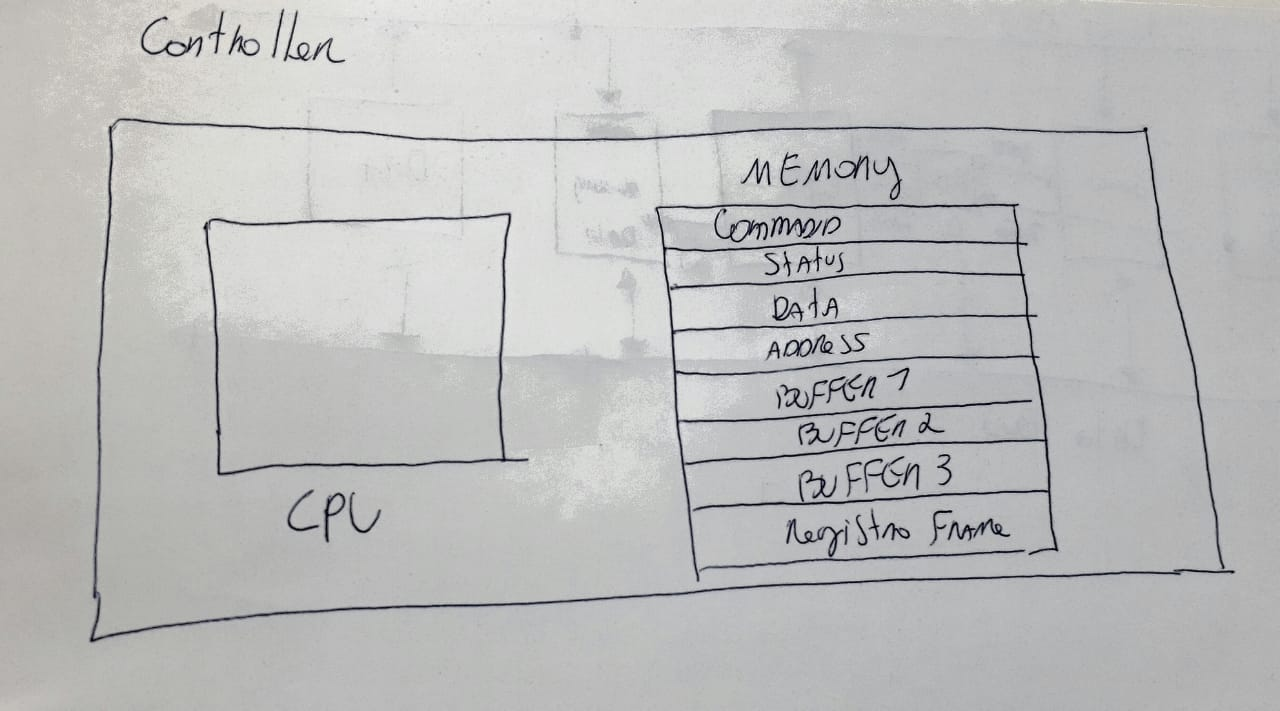
\includegraphics[width=20cm]{foto2.jpeg}

Lo que debe hacer este controlador es lo siguiente:
 \begin{lstlisting} 
    while True:
        if command = enviar:
            while True
                status = enviando
                traspaso_frames_imagen_a_Buffers
                transeferir_primeros_pixeles_a_disco
                transeferir_segundos_pixeles_a_disco
                transeferir_terceros_pixeles_a_disco
                actualizar_registro_frame
                if registro_frame == 0:
                    status = " sin imagenes que enviar"
                    break
                else:
                    actualizar_buffers
        if command = apagar:
            status = apagado
            break
    \end{lstlisting}
                
        
        

% Fin del documento.
\end{document}